\documentclass[a4paper, 11pt]{article}
\usepackage[python]{mypackage}
\usepackage{amsmath}
\usepackage{graphicx}
\usepackage{geometry}
\geometry{scale=0.8}
\usepackage{hyperref}
\usepackage{enumitem}
\usepackage{color}

\setenumerate[1]{itemsep=0pt,partopsep=0pt,parsep=\parskip,topsep=0pt}
\setitemize[1]{itemsep=0pt,partopsep=0pt,parsep=\parskip,topsep=0pt}
\setdescription{itemsep=0pt,partopsep=0pt,parsep=\parskip,topsep=0pt}


\title{
\normalfont \normalsize
\textsc{School of Data and Computer Science, Sun Yat-sen University} \\ [25pt] %textsc small capital letters
\rule{\textwidth}{0.5pt} \\[0.4cm] % Thin top horizontal rule
\huge  E14 BP Algorithm (C++/Python)\\ % The assignment title
\rule{\textwidth}{2pt} \\[0.5cm] % Thick bottom horizontal rule
\author{17341015 Hongzheng Chen}
\date{\normalsize\today}
}

\begin{document}
\maketitle
\tableofcontents
\newpage
\section{Horse Colic Data Set}
The description of the horse colic data set (\url{http://archive.ics.uci.edu/ml/datasets/Horse+Colic}) is as follows:
\begin{figure}[ht]
\centering
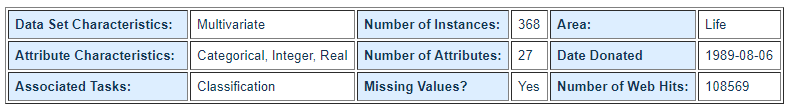
\includegraphics[width=15cm]{horse}
\end{figure}

We aim at trying to predict if a horse with colic will live or die.

Note that we should deal with missing values in the data! Here are some options:
\begin{itemize}
	\item Use the feature’s mean value from all the available data.
	\item Fill in the unknown with a special value like -1.
	\item Ignore the instance.
	\item Use a mean value from similar items.
	\item Use another machine learning algorithm to predict the value.
\end{itemize}

\section{Reference Materials}
\begin{enumerate}
	\item Stanford: \textbf{CS231n: Convolutional Neural Networks for Visual Recognition} by Fei-Fei Li,etc.
	\begin{itemize}
		\item Course website: \url{http://cs231n.stanford.edu/2017/syllabus.html}
		\item Video website: \url{https://www.bilibili.com/video/av17204303/?p=9&tdsourcetag=s_pctim_aiomsg}
	\end{itemize}

	\item \textbf{Machine Learning} by Hung-yi Lee
	\begin{itemize}
		\item Course website: \url{http://speech.ee.ntu.edu.tw/~tlkagk/index.html}
		\item Video website: \url{https://www.bilibili.com/video/av9770302/from=search}
	\end{itemize}
	\item A Simple neural network code template
\begin{lstlisting}
# -*- coding: utf-8 -*
import random
import math

# Shorthand:
# "pd_" as a variable prefix means "partial derivative"
# "d_" as a variable prefix means "derivative"
# "_wrt_" is shorthand for "with respect to"
# "w_ho" and "w_ih" are the index of weights from hidden to output layer neurons and input to hidden layer neurons respectively

class NeuralNetwork:
    LEARNING_RATE = 0.5
    def __init__(self, num_inputs, num_hidden, num_outputs, hidden_layer_weights = None, hidden_layer_bias = None, output_layer_weights = None, output_layer_bias = None):
    #Your Code Here

    def init_weights_from_inputs_to_hidden_layer_neurons(self, hidden_layer_weights):
    #Your Code Here

    def init_weights_from_hidden_layer_neurons_to_output_layer_neurons(self, output_layer_weights):
    #Your Code Here

    def inspect(self):
        print('------')
        print('* Inputs: {}'.format(self.num_inputs))
        print('------')
        print('Hidden Layer')
        self.hidden_layer.inspect()
        print('------')
        print('* Output Layer')
        self.output_layer.inspect()
        print('------')

    def feed_forward(self, inputs):
        #Your Code Here

    # Uses online learning, ie updating the weights after each training case
    def train(self, training_inputs, training_outputs):
        self.feed_forward(training_inputs)

        # 1. Output neuron deltas
        #Your Code Here
        # ∂E/∂zⱼ

        # 2. Hidden neuron deltas
        # We need to calculate the derivative of the error with respect to the output of each hidden layer neuron
        # dE/dyⱼ = Σ ∂E/∂zⱼ * ∂z/∂yⱼ = Σ ∂E/∂zⱼ * wᵢⱼ
        # ∂E/∂zⱼ = dE/dyⱼ * ∂zⱼ/∂
        #Your Code Here

        # 3. Update output neuron weights
        # ∂Eⱼ/∂wᵢⱼ = ∂E/∂zⱼ * ∂zⱼ/∂wᵢⱼ
        # Δw = α * ∂Eⱼ/∂wᵢ
        #Your Code Here

        # 4. Update hidden neuron weights
        # ∂Eⱼ/∂wᵢ = ∂E/∂zⱼ * ∂zⱼ/∂wᵢ
        # Δw = α * ∂Eⱼ/∂wᵢ
        #Your Code Here

    def calculate_total_error(self, training_sets):
        #Your Code Here
        return total_error

class NeuronLayer:
    def __init__(self, num_neurons, bias):

        # Every neuron in a layer shares the same bias
        self.bias = bias if bias else random.random()

        self.neurons = []
        for i in range(num_neurons):
            self.neurons.append(Neuron(self.bias))

    def inspect(self):
        print('Neurons:', len(self.neurons))
        for n in range(len(self.neurons)):
            print(' Neuron', n)
            for w in range(len(self.neurons[n].weights)):
                print('  Weight:', self.neurons[n].weights[w])
            print('  Bias:', self.bias)

    def feed_forward(self, inputs):
        outputs = []
        for neuron in self.neurons:
            outputs.append(neuron.calculate_output(inputs))
        return outputs

    def get_outputs(self):
        outputs = []
        for neuron in self.neurons:
            outputs.append(neuron.output)
        return outputs

class Neuron:
    def __init__(self, bias):
        self.bias = bias
        self.weights = []

    def calculate_output(self, inputs):
    #Your Code Here

    def calculate_total_net_input(self):
    #Your Code Here

    # Apply the logistic function to squash the output of the neuron
    # The result is sometimes referred to as 'net' [2] or 'net' [1]
    def squash(self, total_net_input):
    #Your Code Here

    # Determine how much the neuron's total input has to change to move closer to the expected output
    #
    # Now that we have the partial derivative of the error with respect to the output (∂E/∂yⱼ) and
    # the derivative of the output with respect to the total net input (dyⱼ/dzⱼ) we can calculate
    # the partial derivative of the error with respect to the total net input.
    # This value is also known as the delta (δ) [1]
    # δ = ∂E/∂zⱼ = ∂E/∂yⱼ * dyⱼ/dzⱼ
    #
    def calculate_pd_error_wrt_total_net_input(self, target_output):
    #Your Code Here

    # The error for each neuron is calculated by the Mean Square Error method:
    def calculate_error(self, target_output):
    #Your Code Here

    # The partial derivate of the error with respect to actual output then is calculated by:
    # = 2 * 0.5 * (target output - actual output) ^ (2 - 1) * -1
    # = -(target output - actual output)
    #
    # The Wikipedia article on backpropagation [1] simplifies to the following, but most other learning material does not [2]
    # = actual output - target output
    #
    # Alternative, you can use (target - output), but then need to add it during backpropagation [3]
    #
    # Note that the actual output of the output neuron is often written as yⱼ and target output as tⱼ so:
    # = ∂E/∂yⱼ = -(tⱼ - yⱼ)
    def calculate_pd_error_wrt_output(self, target_output):
    #Your Code Here

    # The total net input into the neuron is squashed using logistic function to calculate the neuron's output:
    # yⱼ = φ = 1 / (1 + e^(-zⱼ))
    # Note that where ⱼ represents the output of the neurons in whatever layer we're looking at and ᵢ represents the layer below it
    #
    # The derivative (not partial derivative since there is only one variable) of the output then is:
    # dyⱼ/dzⱼ = yⱼ * (1 - yⱼ)
    def calculate_pd_total_net_input_wrt_input(self):
    #Your Code Here

    # The total net input is the weighted sum of all the inputs to the neuron and their respective weights:
    # = zⱼ = netⱼ = x₁w₁ + x₂w₂ ...
    #
    # The partial derivative of the total net input with respective to a given weight (with everything else held constant) then is:
    # = ∂zⱼ/∂wᵢ = some constant + 1 * xᵢw₁^(1-0) + some constant ... = xᵢ
    def calculate_pd_total_net_input_wrt_weight(self, index):
    #Your Code Here

# An example:

nn = NeuralNetwork(2, 2, 2, hidden_layer_weights=[0.15, 0.2, 0.25, 0.3], hidden_layer_bias=0.35, output_layer_weights=[0.4, 0.45, 0.5, 0.55], output_layer_bias=0.6)
for i in range(10000):
    nn.train([0.05, 0.1], [0.01, 0.99])
    print(i, round(nn.calculate_total_error([[[0.05, 0.1], [0.01, 0.99]]]), 9))
\end{lstlisting}

\end{enumerate}
\section{Tasks}
\begin{itemize}
	\item Given the training set \texttt{horse-colic.data} and the testing set \texttt{horse-colic.test}, implement the BP algorithm and establish a neural network to predict if horses with colic will live or die. In addition, you should calculate the accuracy rate.
	\item Please submit a file named \texttt{E14\_YourNumber.pdf} and send it to \texttt{ai\_201901@foxmail.com}
\end{itemize}

\section{Codes and Results}


\end{document}